% VUT FIT MITAI
% MSZ 2021/2022
% Author: Vladimir Dusek
% Login: xdusek27

%%%%%%%%%%%%%%%%%%%%%%%%%%%%%%%%%%%%%%%%%%%%%%%%%%%%%%%%%%%%%%%%%%%%%%%%%%%%%%%%

% Path to figures
\graphicspath{{pds/rizeni_toku_a_prevence_zahlceni/figures}}

%%%%%%%%%%%%%%%%%%%%%%%%%%%%%%%%%%%%%%%%%%%%%%%%%%%%%%%%%%%%%%%%%%%%%%%%%%%%%%%%

\chapter{PDS -- Řízení toku dat (flow-control) a prevence zahlcení (congestion-control) na transportní vrstvě (MP-TCP, QUIC, SCTP, DCCP).}

%%%%%%%%%%%%%%%%%%%%%%%%%%%%%%%%%%%%%%%%%%%%%%%%%%%%%%%%%%%%%%%%%%%%%%%%%%%%%%%%

\section{Zdroje}

\begin{compactitem}
    \item \path{02-transportni-protokoly.pdf}
    \item \path{PDS_2021-02-19.mp4}
\end{compactitem}

%%%%%%%%%%%%%%%%%%%%%%%%%%%%%%%%%%%%%%%%%%%%%%%%%%%%%%%%%%%%%%%%%%%%%%%%%%%%%%%%

\section{Úvod a kontext}

\textit{Viz. \uv{Úvod a kontext} v~předchozích otázkách z~tohoto předmětu.}

\paragraph*{Transportní vrstva} Transportní vrstva je název čtvrté vrstvy modelu vrstvové síťové architektury (ISO/OSI model). Leží mezi vrstvou síťovou (L3) a aplikační (L7). \begin{compactitem}
    \item Činnost na straně odesílatele: obdrží data z aplikační vrstvy, nasegmentuje je a ke každému segmentu/datagramu přidá L4 hlavičku.
    \item Činnost na straně příjemce: obdrží segmenty/datagramy, které uspořádá do správného pořadí (\textit{out-of-order} doručení), předá je aplikační vrstvě.
    \item Komunikace mezi vrstvami L4 a L7 probíhá pomocí socketů.
    \item Zodpovědnost za \textit{end-to-end} spojení.
    \item Adresuje aplikace pomocí portových čísel.
    \item \textit{Quality of Service}~--~zotavení se z chyb, spolehlivost, řízení toku, řízení zahlcení.
\end{compactitem}

\paragraph*{Multi homing}~--~Využítí více bodů připojení zároveň (pro jednu komunikaci). Pokud je podporováno a změní se IP adresa, nemusí se navázat nové spojení.

\paragraph*{\textit{Connection-oriented}}~--~Typ spojení, kdy je nejprve nutné, navázat komunikaci. Typicky tři fáze: navázání spojení, přenos dat, ukončení spojení.

\paragraph*{\textit{Connection-less}}~--~Typ spojení, které nerozlišuje jestli spojení existuje, nebo nikoliv. Pouze fáze přenosu dat.

\paragraph*{Round trip time (RTT)} RTT je doba, která uplyne od vyslání paketu z jednoho komunikujícího uzlu k druhému po návrat potvrzení zpátky na první uzel.

\paragraph*{bandwith, throughput, goodput} \begin{compactitem}
    \item \textit{Bandwith}~--~šířka pásma (maximální přenos dat danou cestou v jeden moment)
    \item \textit{Throughput}~--~propustnost komunikace na úrovni protokolu
    \item \textit{Goodput}~--~propustnost komunikace na úrovni aplikace (throughput $-$ režie)
\end{compactitem}

\paragraph*{Bitové chyby} \begin{compactitem}
    \item \uv{Přeskočení bitu} (\textit{bit swapping}), jde o chyby na úrovni zpracování informace uzlem v síti (typicky spojené s přenosovým médiem)
    \item Zabýváme se jimi na úrovni L2
    \item Řešením je obvykle redundance (Hammingův kód, CRC, Viterbiho algoritmus, \dots)
\end{compactitem}

\begin{figure}[H]
    \centering
    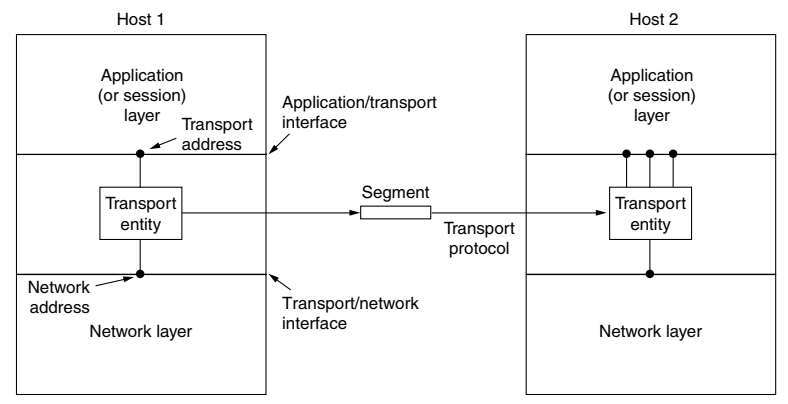
\includegraphics[width=1\linewidth]{l4.png}
    \caption{Transportní vrstva (L4).}
\end{figure}

%%%%%%%%%%%%%%%%%%%%%%%%%%%%%%%%%%%%%%%%%%%%%%%%%%%%%%%%%%%%%%%%%%%%%%%%%%%%%%%%

\section{Paketové chyby}

\begin{compactitem}
    \item Jde o chyby na úrovni přenosu informace mezi dvěma uzly.
    \item Zabýváme se jimi na transportní vrstvě.
    \item Řešením je obvykle znovuzaslání paketu.
    \item Můžeme měřit: \begin{compactitem}
        \item PER (\textit{packet error rate}) $$PER = \frac{\text{pocet chybnych paketu}}{\text{pocet prenesenych paketu}}$$
        \item BER (\textit{bit error rate}) $$BER = \frac{\text{pocet chybnych bitu}}{\text{pocet prenesenych bitu}}$$
    \end{compactitem}
    \item Dále jsou představeny druhy paketových chyb.
\end{compactitem}

\paragraph*{Ztráta (zpoždění) paketu} Jak může dojít ke ztrátě (zpoždění) paketu? \begin{compactitem}
    \item Neopravitelná bitová chyba (rámec je zahozen na L2)
    \item Zahlcení linky (směrovače jsou přetíženy a některé pakety zahazují)
    \item Špatné směrovací tabulky (paket jde špatnou cestou, nebo cyklí a vyprší mu TTL)
\end{compactitem}

\paragraph*{Ztráta fragmentovaných dat} Fragment se může ztratit ze stejného důvodu jako standardní nefragmentovaný paket.

\paragraph*{Duplicita paketu} Příjemce obdržuje stále paket se stejným sekvenčním číslem. Odesílatel si myslí, že se paket k příjemci nikdy nedostal. Proč? \begin{compactitem}
    \item Ztratí se potvrzení o přijetí paketu.
\end{compactitem}

\paragraph*{Vložení paketu} Příjemce obdrží paket, který do spojení nepatří. Jak k tomu může dojít? \begin{compactitem}
    \item Přijetí zpožděného paketu, který dorazil až po skončení jednoho a začátku dalšího separátního datového toku.
    \item Podvrhávání paketu útočníkem snažícím se narušit integritu sítě.
    \item Paket je chybou \uv{zvláštně zmrzačen} tak, že chybu nelze rozpoznat (např. je změněm bit v cílové IP adrese) a je směrován jinému příjemci.
\end{compactitem}

\paragraph*{Změna pořadí} Vychází z designu počítačových sítí, kdy paketu mohou proudit různými cestami a s různým zpožděním. Data jsou \textit{out-of-order} a příjemce je musí přeuspořádat.

%%%%%%%%%%%%%%%%%%%%%%%%%%%%%%%%%%%%%%%%%%%%%%%%%%%%%%%%%%%%%%%%%%%%%%%%%%%%%%%%

\section{Řízení toku}

Řízení toku (\textit{flow control}) je řízení komunikaci mezi dvěma uzly na straně koncového systému. Řízení zahlcení (\textit{congestion control}) je řízení komunikace v rámci sítě. Alternativně, se za řízení toku považuje koncept detekce a korekce paketových chyb. Často jsou tyto termíny vykládány různě.

\subsection{Detekce paketové chyby}

Paketové chyby detekujeme pomocí sekvenčních čísel. Sekvenční číslo je jedinečný identifikátor paketu v rámci datového toku, který identifikuje jeho pořadí. Tímto poznáme ztrátu, duplicitu i změnu pořadí.

\medskip\noindent Jak rozpoznat ztrátu od zpoždění? \begin{compactitem}
    \item \textbf{Timeout}~--~Může být fixní, ale v lepším případě se odvozuje od RTT.
    \item \textbf{Negativní potvrzování}~--~Paket jsem dostal (ACK) vs. paket jsem nedostal (NACK). Pokud je příčina zpoždění zahlcení, tak tento přístup linku ještě více zahltí.
\end{compactitem}

\subsection{Korekce paketových chyb}

Pokud paket nedorazil, odesílatel ho pošle znovu. Tzv. \textit{Automatic Repeat/Request} (ARQ)~--~Čeká se na ACK, když nepřijde do timeoutu, dojde k znovuzaslání. Princip tzv. klouzavého okna (\textit{sliding window}). Existují 3 strategie.

\paragraph*{Stop and wait} \begin{compactitem}
    \item Klouzavé okno o velikosti 1.
    \item Odesílatel pošle paket a čeká na potvrzení. Po přijetí potvrzení pošle další paket.
    \item Špatná efektivita využití pásma.
\end{compactitem}

\paragraph*{Go back n} \begin{compactitem}
    \item Buffer na straně odesílatele.
    \item Příjemce potvrzuje naposledy přijatým paketem (např. příjemce pošle ACK2 znamená, že dostal pakety 0, 1, 2).
    \item Plýtvání při znovuzaslání (např. odesílatel pošle 5 paketů, ztratí se první, musí poslat znovu všech 5).
\end{compactitem}

\paragraph*{Selective repeat} \begin{compactitem}
    \item Buffery jsou na obou stranách.
    \item Efektivní využítí šířky pásma, ale složitější implementace.
    \item Příjemce potvrzuje: \begin{compactitem}
        \item Fast Retransmit -- Příjemce posílá potvrzení s naposledy přijatým paketem.
        \item Bitová maska -- V ACK je zavedeno další políčko (bitová maska), které obsahuje informace o tom, co příjemce přijal a co ne.
        \item NACK -- Příjemce posílá ACK, pokud balík dostal a NACK, pokud nikoliv.
    \end{compactitem}
\end{compactitem}

%%%%%%%%%%%%%%%%%%%%%%%%%%%%%%%%%%%%%%%%%%%%%%%%%%%%%%%%%%%%%%%%%%%%%%%%%%%%%%%%

\section{Řízení zahlcení}

Zahlcení je detekováno, co se s tím dá dělat? \begin{compactitem}
    \item Zvýšit kapacitu sítě,
    \item Snížit množství provozu.
\end{compactitem}

\noindent Jak se to dá dělat? \begin{compactitem}
    \item Opravit zahlcený provoz (\textit{repair})~--~Je detekováno zahlcení a řešíme, co budeme dělat.
    \item Předcházet problému zahlcení (\textit{avoidance})~--~Snažíme se zahlcení předcházet (prevence).
\end{compactitem}

\subsection{Zahazování paketů (opravování provozu)}

Každý uzel (najčastěji směrovač) v síti kontroluje délku své fronty, pokud příliš narůstá, tak začne preventivně některé pakety zahazovat (to však vede k jejich znovuzaslání).

\paragraph*{RED (\textit{Random Early Detection})} Algoritmus RED sleduje velikost fronty a zahazuje pakety na základě pravděpodobnosti. Pokud je fronta téměř prázdná, pravděpodobnost zahození je 0. Jak fronta roste, roste i pravděpodobnost zahození příchozího paketu. Když je fronta plná, pravděpodobnost dosáhne hodnoty 1 a všechny příchozí pakety jsou zahazovány.

\begin{figure}[H]
    \centering
    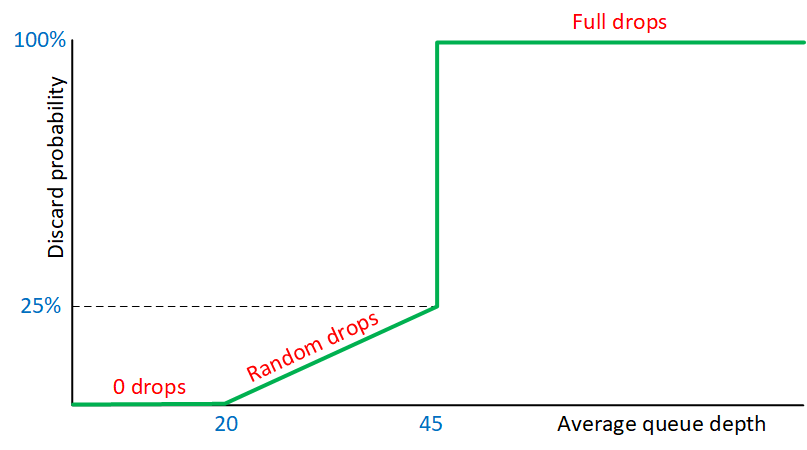
\includegraphics[width=0.9\linewidth]{red.png}
    \caption{Vizualizace RED.}
\end{figure}

\paragraph*{WRED (\textit{Weighted Random Early Detection})} Algoritmus WRED je rozšířením RED o přidání váh pro jednotlivé třídy paketů (máme frontu pro každou třídu). WRED nezahazuje všechny pakety se stejnou pravděpodobností, ale rozlišuje jejich důležitost (pomocí hodnot IP precedence nebo DSCP). Některé pakety chceme prioritizovat, např. VoIP (\textit{Voice over Internet Protocol}), RTP (\textit{Real-time Transport Protocol}).

\begin{figure}[H]
    \centering
    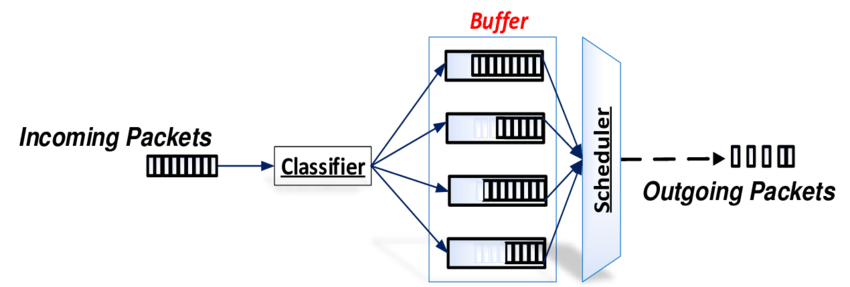
\includegraphics[width=1\linewidth]{wred.png}
    \caption{Vizualizace WRED.}
\end{figure}

\subsection{Choke pakety (opravování provozu)}

Příjemce v síti má problém zpracovávat provoz (nestíhá), tak dá vědět odesílateli (odešle choke paket), aby zpomalil.

\paragraph*{Plain choke packets} Viz obrázek~\ref{pds_choke_packets}. Uzel D detekuje zahlcení způsobené provozem od A. Uzel D pošle choke paket A. Proti zahlcení \uv{zabojuje} pouze odesílatel (A).

\paragraph*{Hop-by-hop choke packets} Viz obrázek~\ref{pds_choke_packets}. Uzel D detekuje zahlcení způsobené provozem od A. Uzel D pošle choke paket A. Každý uzel po cestě \uv{bojuje} proti zahlcení (F, E, A).

\begin{figure}[H]
    \centering
    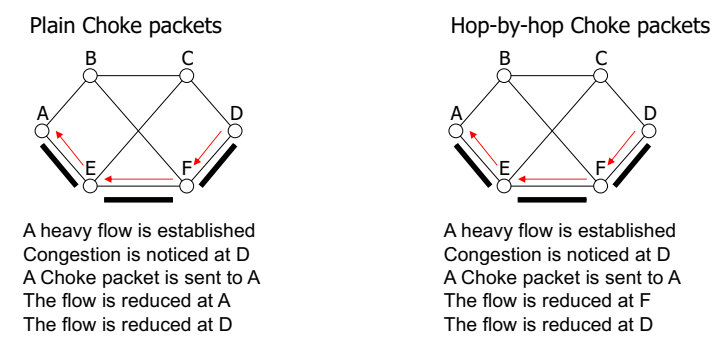
\includegraphics[width=1\linewidth]{choke_packets.png}
    \caption{\textit{Plain choke packets} vs. \textit{hop-by-hop choke packets}.}
    \label{pds_choke_packets}
\end{figure}

\subsection{Ořezání a rozložení provozu (předcházení zahlcení)}

Jedná se o předcházení zahlcení ze strany odesílatele. Odesílatel je \uv{ohleduplný} a myslí na to, aby příjemce nebyl zahlcen. Odesílatel má pevně stanovenou hranici kolik můze maximálně posílat. Implementace pomocí tzv. \textit{token bucket}.

\paragraph*{Ořezání provozu (\textit{policing})} Cokoliv nad hranici je \uv{oříznuto} a zahozeno.

\paragraph*{Rozložení provozu (\textit{shaping})} Cokoliv nad hranici je uloženo do bufferu a odesláno později, až je menší provoz.

\begin{figure}[H]
    \centering
    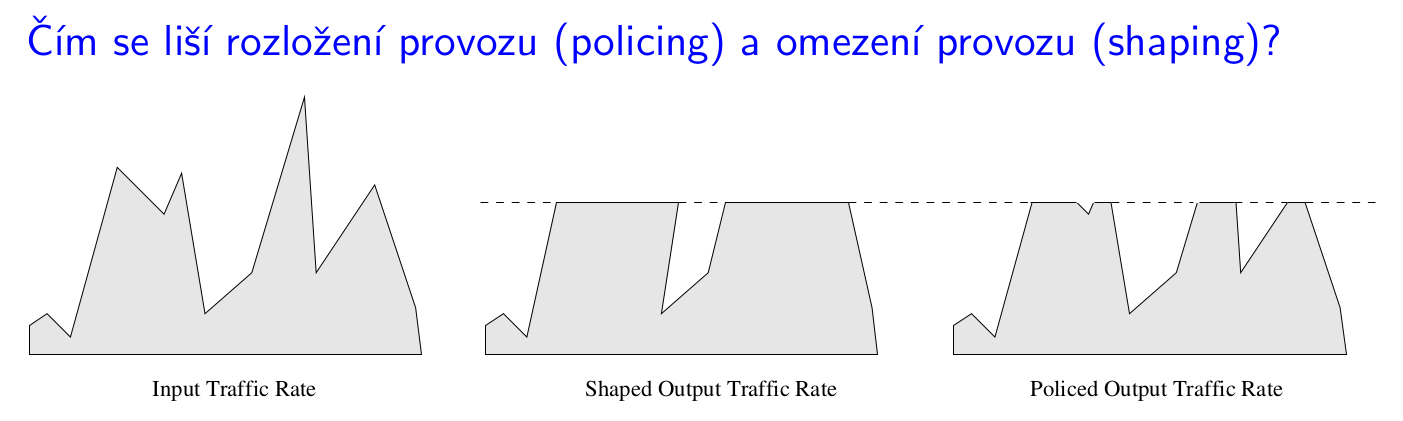
\includegraphics[width=1\linewidth]{traffic_policing_and_shaping.png}
    \caption{Ořezání provozu vs rozložení provozu.}
\end{figure}

\subsection{Rezervace (předcházení zahlcení)}

Zařízení v síti (směrovače) jsou schopni se domluvit a vytvořit si tzv. \uv{virtuální okruh} pro konkrétní komunikaci. Každé zařízení na okruhu ví o provozu a rezervuje potřebné pásmo (předem se deklarují kapacity). Je nutné více signaliace (režie).

\begin{figure}[H]
    \centering
    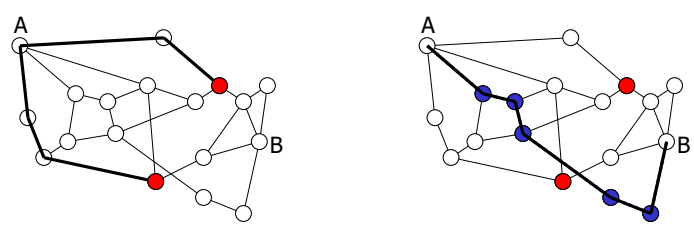
\includegraphics[width=1\linewidth]{rezervace.png}
    \caption{Příklad rezervace.}
\end{figure}

%%%%%%%%%%%%%%%%%%%%%%%%%%%%%%%%%%%%%%%%%%%%%%%%%%%%%%%%%%%%%%%%%%%%%%%%%%%%%%%%

\section{TCP (\textit{Transmission Control Protocol})}

\begin{compactitem}
    \item Garantuje spolehlivé doručení.
    \item Garantuje doručení v pořadí.
    \item Řízení toku a zahlcení.
    \item \textit{Connection-oriented}~--~Navázání spojení pomocí \textit{three-way handshake}.
    \item Pracuje s \textit{byte stream}~--~nezohledňuje hranice aplikačních dat.
    \item Sekvenční číslo závisí na tom, kolik bajtů se posílá. Např. $seq=92, data=8\,B$, $seq=100, data=20\,B$, $seq=120, data=13\,B$, \dots
\end{compactitem}

\begin{figure}[H]
    \centering
    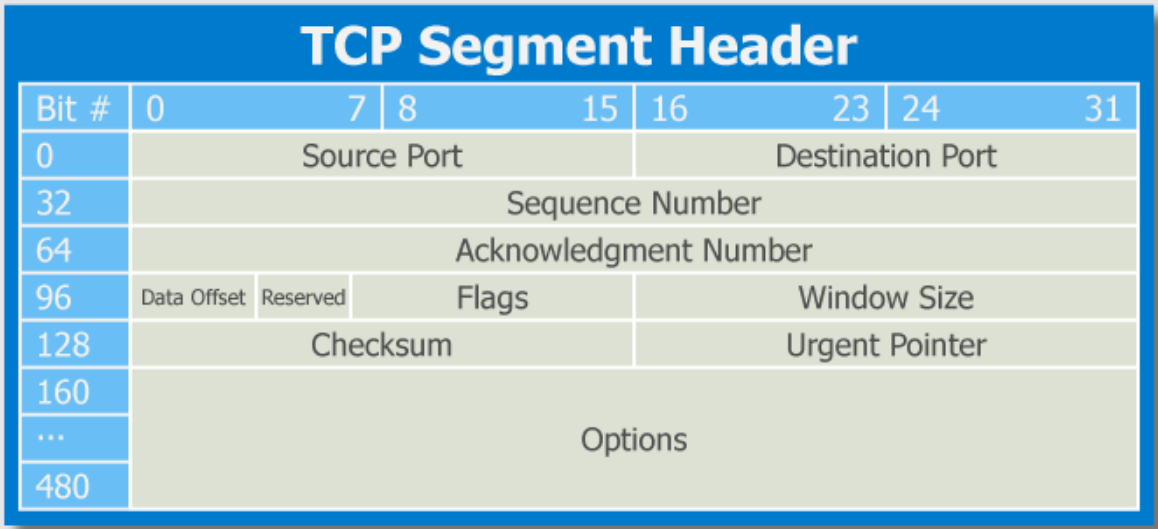
\includegraphics[width=0.75\linewidth]{tcp_header.png}
    \caption{Hlavička TCP.}
\end{figure}

\paragraph*{Řízení toku a zahlcení} V TCP jsou rozlišovány 3 fáze přenosu dat. \begin{compactitem}
    \item \textit{Slow start}~--~Exponenciální zvyšování rychlosti odesílání až po dosažení nějaké hranice.
    \item \textit{Congestion avoidance (additive increase)}~--~Lineární zvyšování počtu odeslaných paketů.
    \item \textit{Congestion avoidance (multiplicative decrease)}~--~Skokové snížení rychlosti odesílání. Nastane, pokud je detekována ztráta paketu.
\end{compactitem}

\noindent V TCP existuje spoustu algoritmů pro řízení toku a zahlcení, které implementují tento princip (Tahoe, Reno, New Reno, Vegas, CUBIC, Westwood, \dots).

\begin{figure}[H]
    \centering
    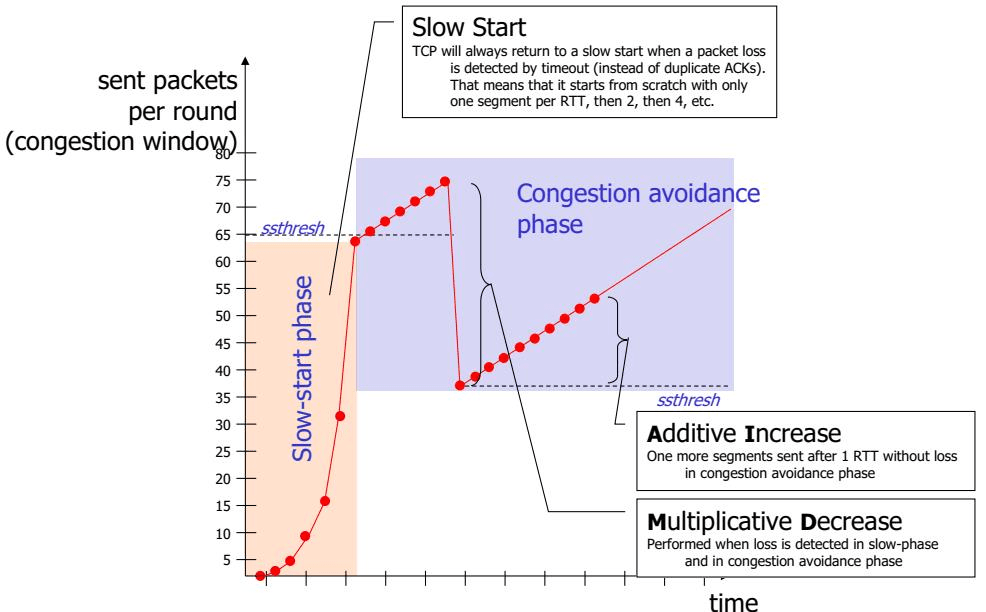
\includegraphics[width=1\linewidth]{ss_ca_ai_md.png}
    \caption{Jednotlivé fáze řízení zahlcení v TCP.}
\end{figure}

\paragraph*{Nevýhody a problémy} \begin{compactitem}
    \item Nepodporuje \textit{multi homing}.
    \item \textit{Head of line blocking}~--~Pokud dojde ke ztrátě paketu, tak vše za ním je pozdrženo
    \item Velká režie potvrzování (až 35\,\% veškerého provozu je režie)
\end{compactitem}

\begin{figure}[H]
    \centering
    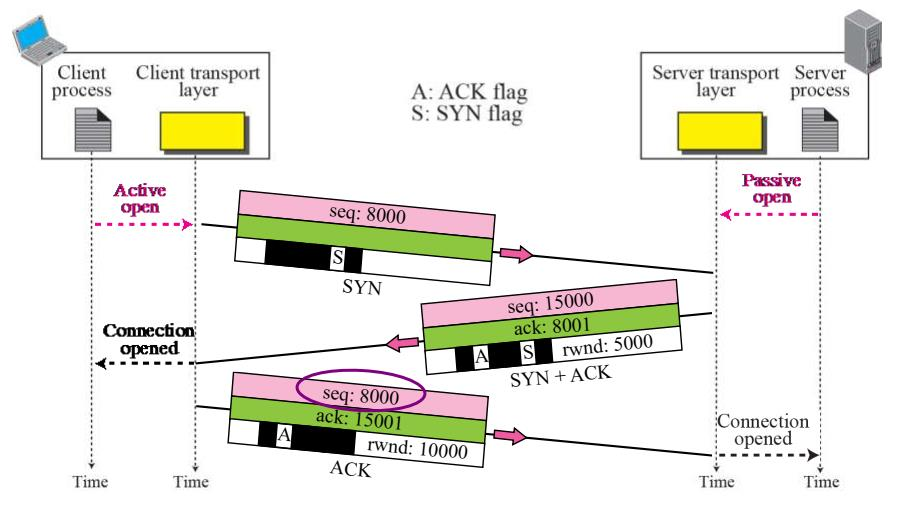
\includegraphics[width=1\linewidth]{tcp_zahajeni_spojeni.png}
    \caption{Zahájení spojení pomocí tzv. \textit{Three-Way Handshake}.}
\end{figure}

%%%%%%%%%%%%%%%%%%%%%%%%%%%%%%%%%%%%%%%%%%%%%%%%%%%%%%%%%%%%%%%%%%%%%%%%%%%%%%%%

\section{UDP (\textit{User Datagram Protocol})}

\begin{compactitem}
    \item Negarantuje spolehlivé doručení (\textit{best effort}).
    \item Negarantuje doručení v pořadí.
    \item \textit{Connection-less}.
    \item Pracuje s \textit{byte stream}~--~nezohledňuje hranice aplikačních dat.
    \item Má minimální režii.
\end{compactitem}

\begin{figure}[H]
    \centering
    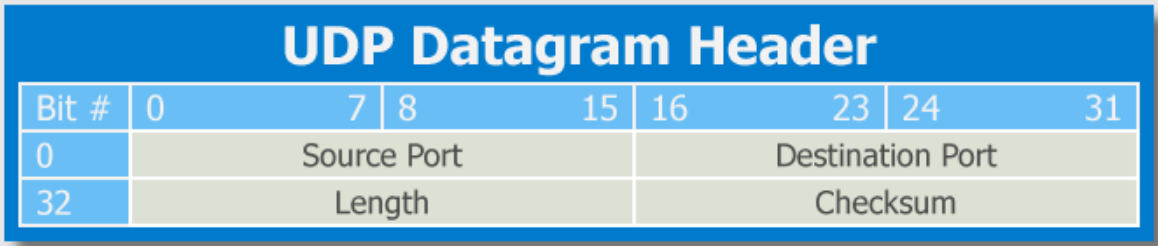
\includegraphics[width=0.75\linewidth]{udp_header.png}
    \caption{Hlavička UDP.}
\end{figure}

\begin{figure}[H]
    \centering
    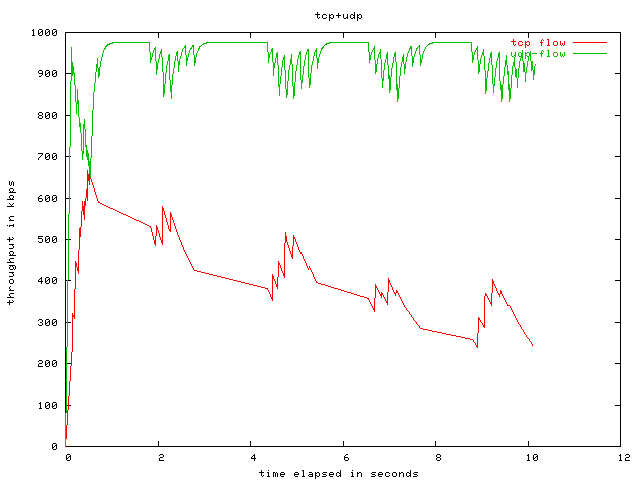
\includegraphics[width=1\linewidth]{udp_problem.png}
    \caption{Problém UDP, kdy si pro sebe zabere celé pásmo, protože TCP se chová \uv{zodpovědně} a snižuje svůj provoz.}
\end{figure}

%%%%%%%%%%%%%%%%%%%%%%%%%%%%%%%%%%%%%%%%%%%%%%%%%%%%%%%%%%%%%%%%%%%%%%%%%%%%%%%%

\section{DCCP (Datagram Congestion Control Protocol)}

\begin{compactitem}
    \item Cílem je zajistit podporu řízení zahlcení pro UDP.
    \item Negarantuje spolehlivé doručení (\textit{best effort}).
    \item Negarantuje doručení v pořadí.
    \item \textit{Connection-oriented}~--~Navázání spojení pomocí \textit{three-way handshake}.
    \item Využití pro audio/video konference.
\end{compactitem}

\begin{figure}[H]
    \centering
    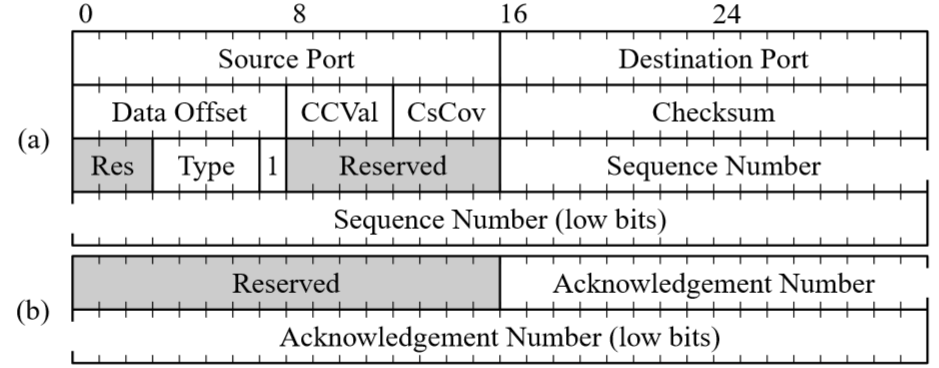
\includegraphics[width=0.75\linewidth]{dccp_header.png}
    \caption{Hlavička DCCP. Sekvenční a potvrzovací čísla souvisí pouze s účtováním provozu kvůli řízení zahlcení, nikoliv pro zajištění spolehlivého přenosu.}
\end{figure}

\begin{figure}[H]
    \centering
    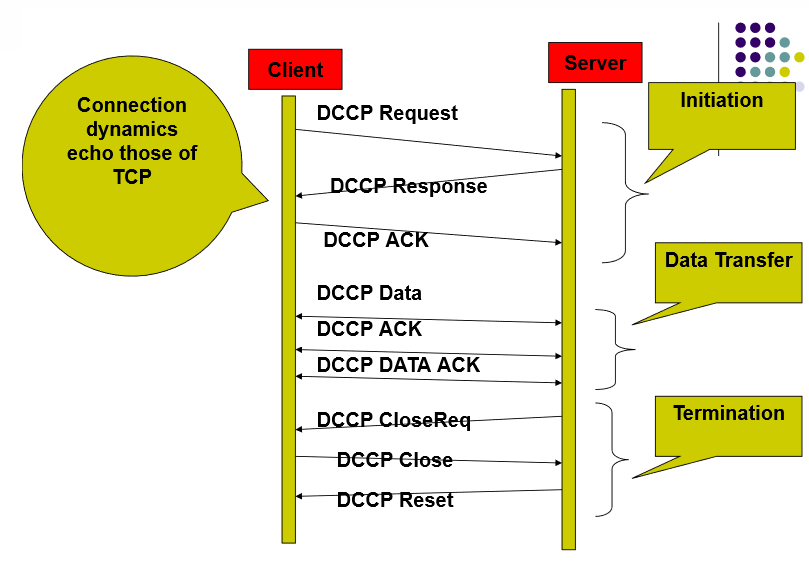
\includegraphics[width=0.75\linewidth]{dccp_spojeni.png}
    \caption{Komunikace pomocí DCCP. Obsahuje několik typů zpráv: Request, Response, ACK, Data, Data ACK, CloseReq, Close, Reset.}
\end{figure}

\paragraph*{Jak je zahlcení realizováno} V potvrzeních se nastavují tzv. ECN (\textit{Explicit Congestion Notification}) bity. Pomocí nich dává příjemce odesílateli vědět, jak moc je zahlcen. V průběhu navazování spojení se pomocí CCID (\textit{Congestion Control ID}) dohodne, jaký typ řízení zahlcení se bude používat (algoritmy jako pro TCP, nebo vlastní).

%%%%%%%%%%%%%%%%%%%%%%%%%%%%%%%%%%%%%%%%%%%%%%%%%%%%%%%%%%%%%%%%%%%%%%%%%%%%%%%%

\section{SCTP (\textit{Stream Control Transmission Protocol})}

\begin{compactitem}
    \item Garantuje spolehlivé doručení.
    \item Garantuje doručení v pořadí.
    \item Pracuje s \textit{message stream}~--~Respektuje hranice aplikačních dat.
    \item \textit{Connection-oriented}~--~Navázání spojení pomocí \textit{four-way handshake}.
    \item \textit{Path MTU discovery}~--~Obrana proti fragmentaci (od zdroje k cíli jsou prozkoumány MTU všech uzlů).
    \item Netrpí problémem \textit{head of line blocking}.
    \item Podporuje \textit{multi homing}.
    \item Řízení zahlceni.
    \item Aplikace je třeba přeprogramovat, aby místo TCP socketů využívali SCTP sockety.
\end{compactitem}

\begin{figure}[H]
    \centering
    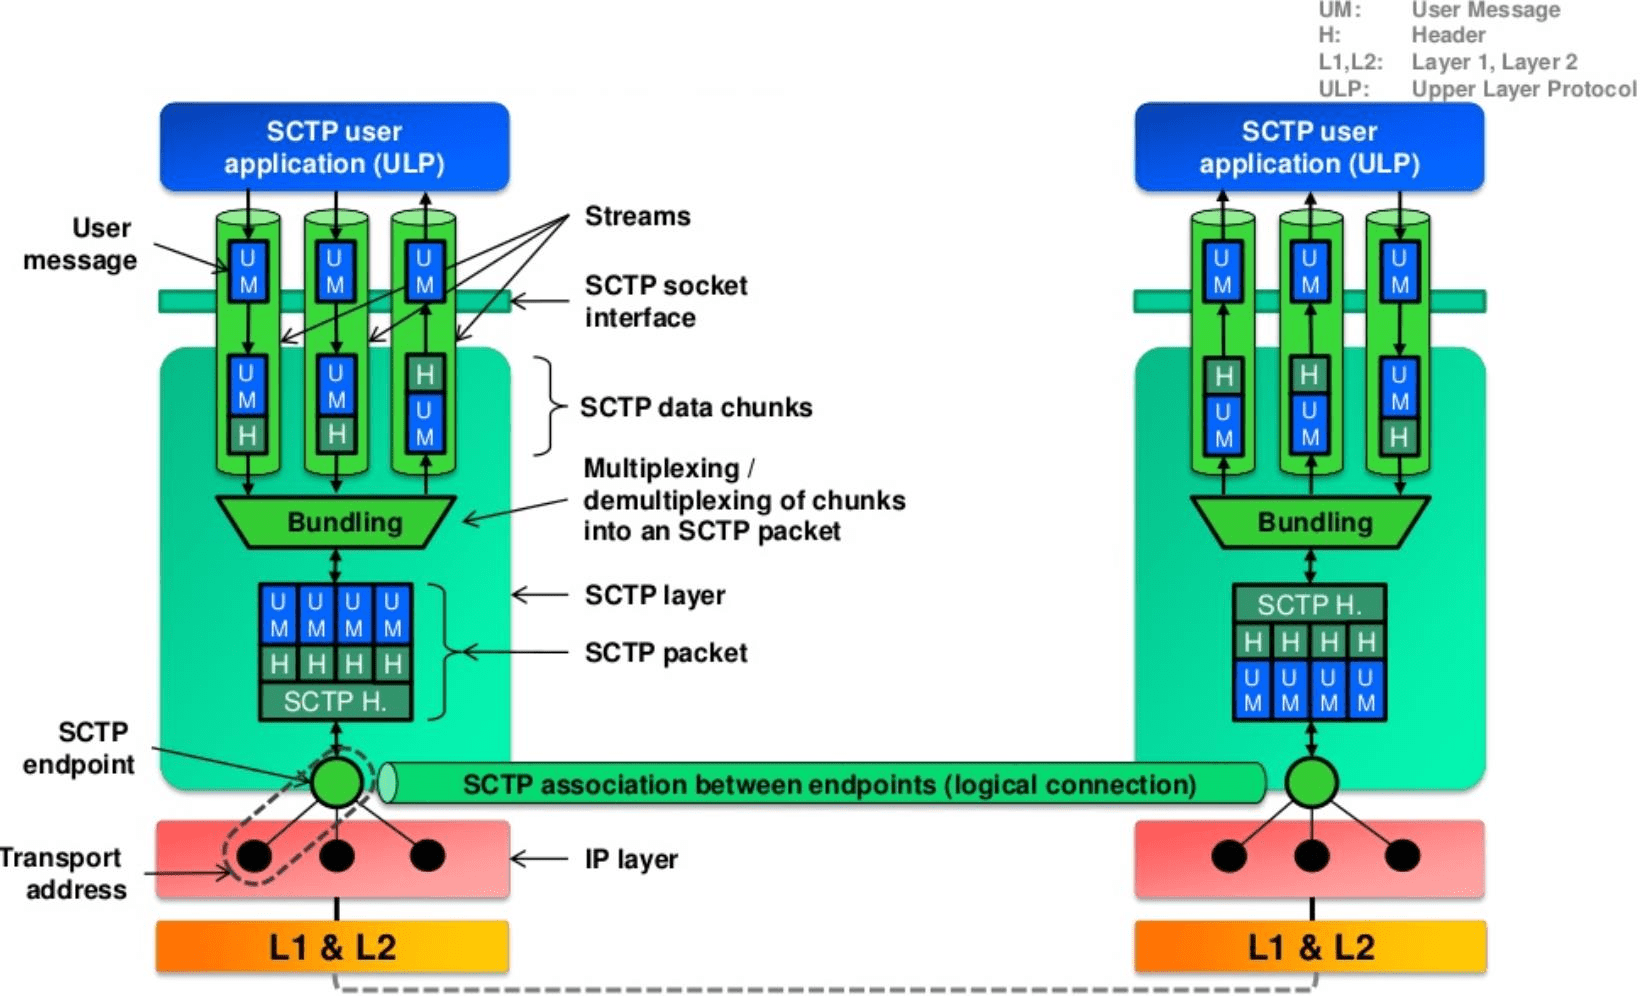
\includegraphics[width=1\linewidth]{sctp_komunikace.png}
    \caption{Komunikace pomocí SCTP. Komunikace s aplikací probíhá přes sockety. Každé aplikační zprávě je přidán základní hlavičkou~--~vzniká \textit{data chunk}. Několik data chunku je zabaleno dohromady a opatřeno SCTP hlavičkou~--~vzniká SCTP paket. Ten je poté možno posílat přes více IP spojení.}
\end{figure}

\begin{figure}[H]
    \centering
    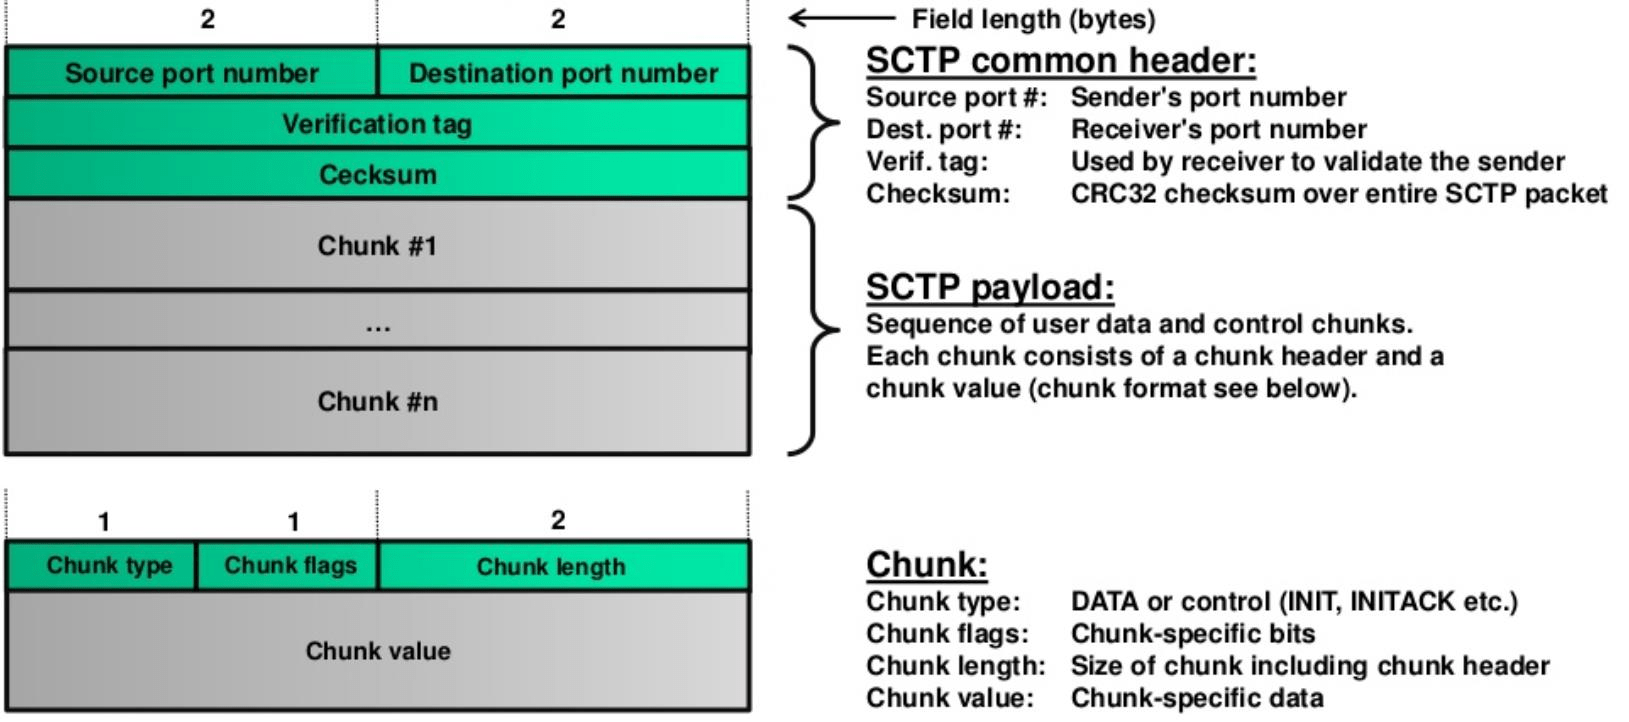
\includegraphics[width=1\linewidth]{sctp_header_1.png}
    \caption{Hlavička SCTP. SCTP paket a \textit{data chunk}.}
\end{figure}

\begin{figure}[H]
    \centering
    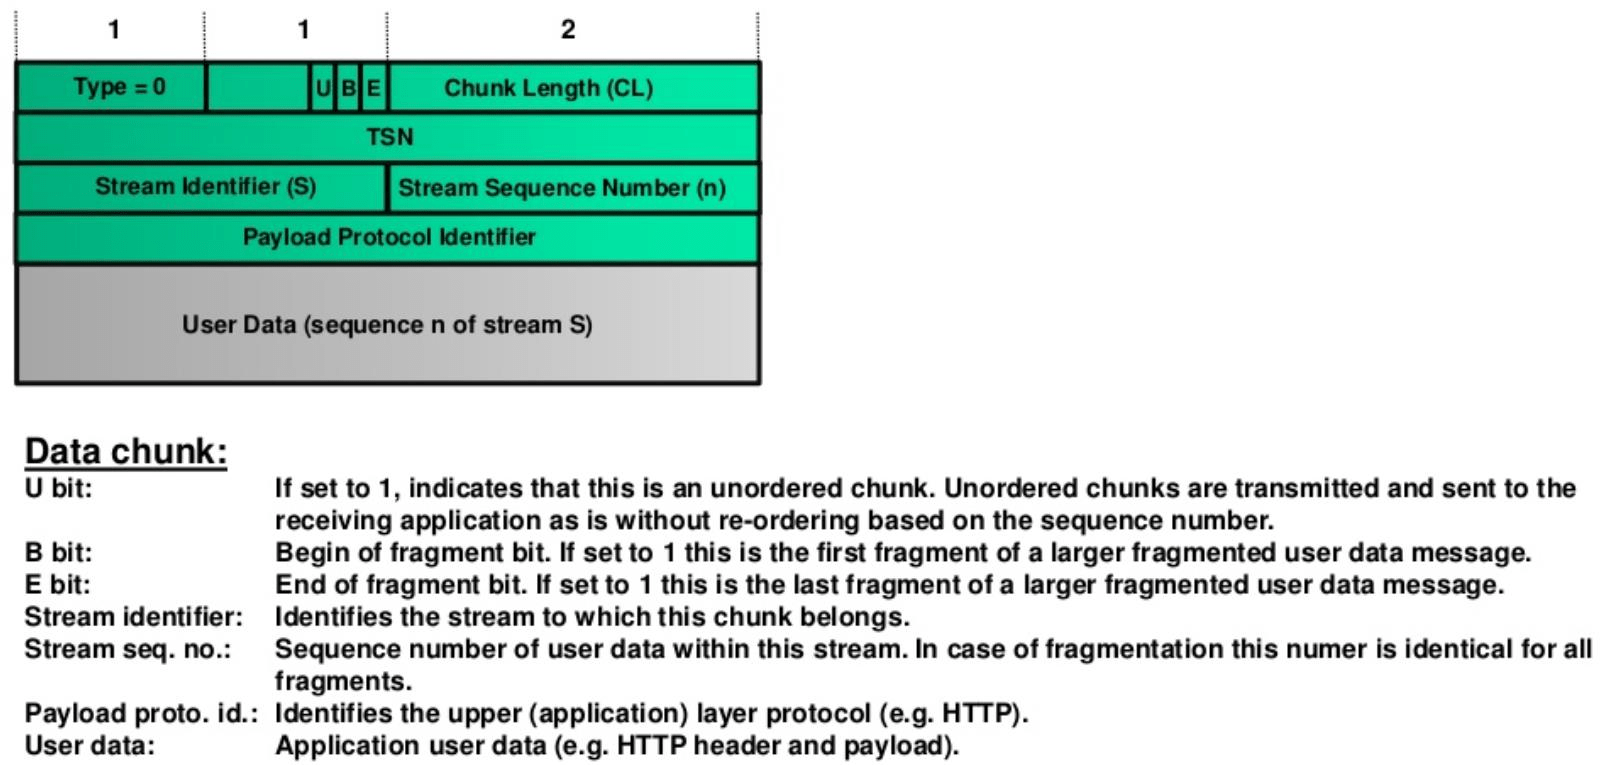
\includegraphics[width=1\linewidth]{sctp_header_2.png}
    \caption{Detailní hlavička \textit{data chunk}. Identifikátor streamu a identifikátor paketu v rámci streamu.}
\end{figure}

% todo flow control?
% slide 93
% EWMA, fast retransmit

\begin{figure}[H]
    \centering
    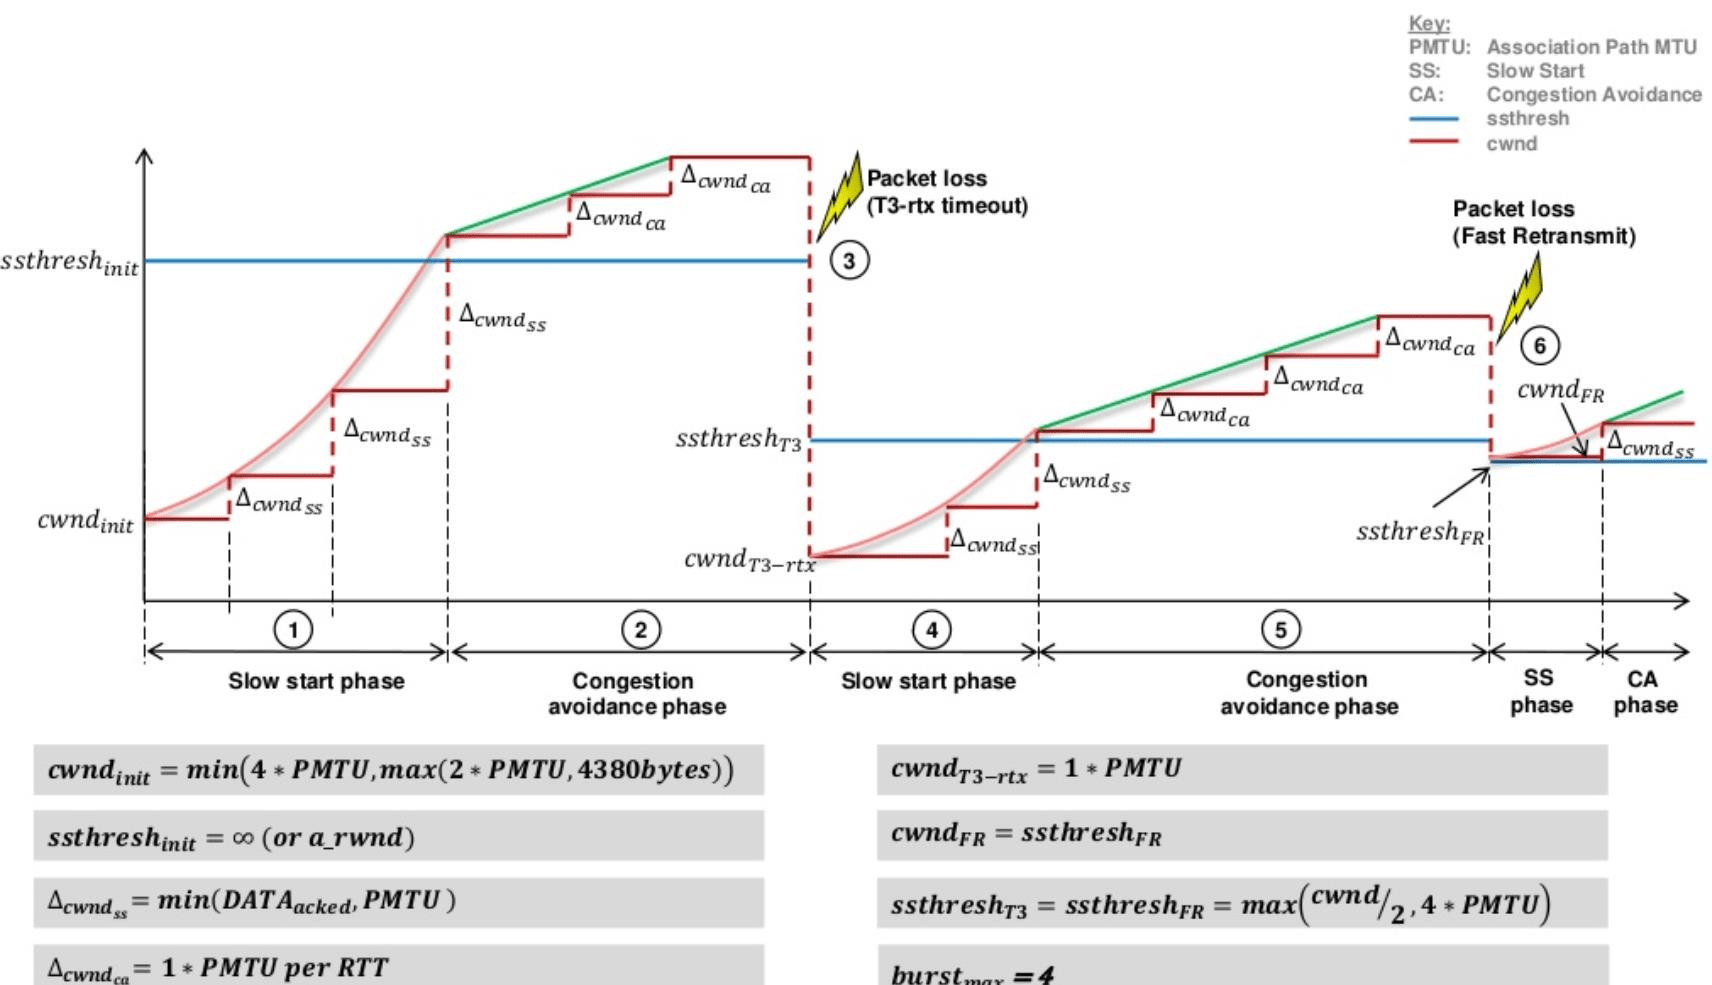
\includegraphics[width=1\linewidth]{sctp_rizeni_zahlceni.png}
    \caption{Řízení zahlcení (\textit{slow start}, \textit{congestion avoidance (additive increase)}, \textit{congestion avoidance (multiplicative decrease)}) je podobné jako TCP Westwood.}
\end{figure}

%%%%%%%%%%%%%%%%%%%%%%%%%%%%%%%%%%%%%%%%%%%%%%%%%%%%%%%%%%%%%%%%%%%%%%%%%%%%%%%%

\section{MP-TCP (\textit{Multipath TCP})}

\begin{compactitem}
    \item Cílem je vzít co nejvíce vlastností z SCTP a poskytnout je v TCP bez toho, aniž by se musely přeprogramovávat aplikace (má obdobné sockety jako TCP).
    \item Má menší signalizační náročnost oproti SCTP.
    \item Chová se jako TCP pouze, podporuje \textit{multi homing} a má vlastní řízení zahlcení.
    \item Rozšíření TCP hlavičky o tzv. \textit{options}.
\end{compactitem}

\begin{figure}[H]
    \centering
    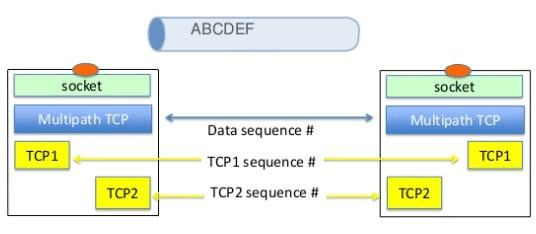
\includegraphics[width=1\linewidth]{mptcp_1.png}
    \caption{MPTCP komunikace, rozdělení aplikačních dat na paralelní TCP streamy. Rozlišujeme datová sekvenční čísla a sekvenční čísla TCP.}
\end{figure}

\begin{figure}[H]
    \centering
    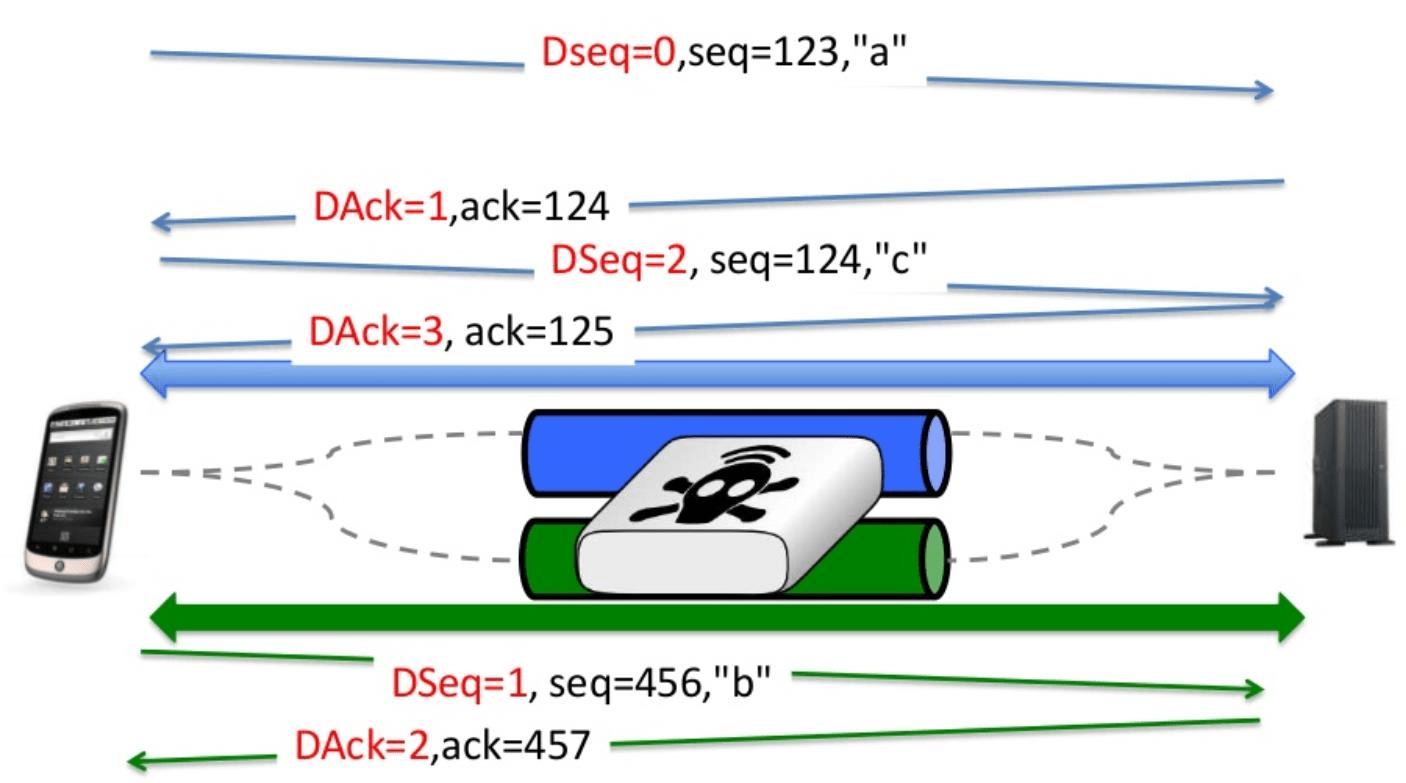
\includegraphics[width=1\linewidth]{mptcp_rizeni_toku.png}
    \caption{MPTCP řízení toku. Dvě TCP komunikace a posílání řetězce \uv{abc}. Navázání spojení podobné jako v TCP. Může vypadnout i celý komunikační kanál.}
\end{figure}

%%%%%%%%%%%%%%%%%%%%%%%%%%%%%%%%%%%%%%%%%%%%%%%%%%%%%%%%%%%%%%%%%%%%%%%%%%%%%%%%

\section{QUIC (\textit{Quick UDP Internet Connections})}

\begin{compactitem}
    \item Motivace pro QUIC: dnes většina provozu probíhá šifrovaně přes HTTPS. Navázání bezpečného HTTPS spojení má velkou režii ($\text{HTTPS} = \text{TCP} + \text{SSL} + \text{HTTP}$). Až $3 \times \text{RTT}$ přes započetím komunikace! \begin{compactitem}
        \item TCP: syn, syn ack, ack
        \item TLS: client hello, server hello, change cipher spec, encrypted handshake message
    \end{compactitem}
    \item Staví nad UDP (aby všechny zařízení v internetu nemuseli implementovat nový transportní protokol).
    \item Paralelní datové streamy, aby bylo zabréněno \textit{head of line blocking}.
    \item Má zabudovanou \textit{Forward Error Correction} (FEC), přidává bitovou redundanci, tím umožňuje velké množství ztracených paketů dopočítat. Pokud to není možný, tak \uv{chytrý} selective repeat.
\end{compactitem}

\begin{figure}[H]
    \centering
    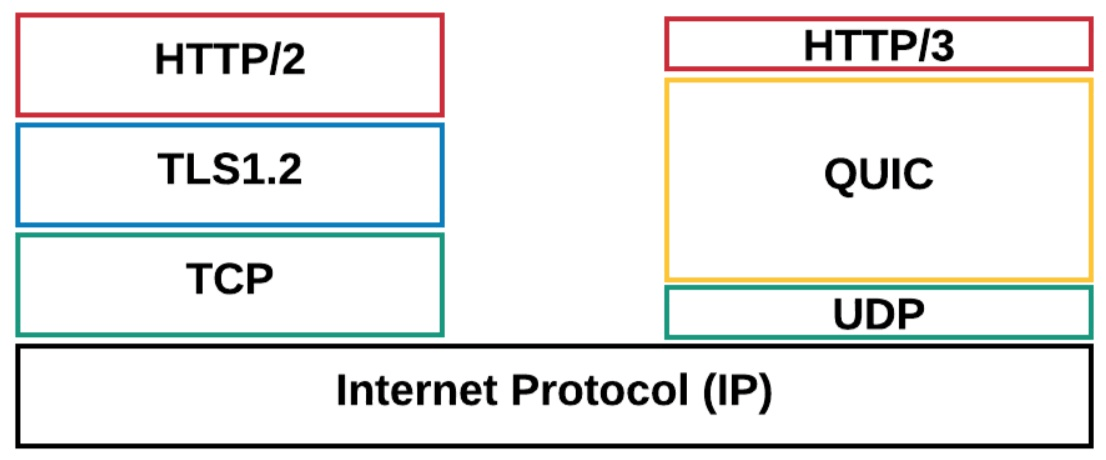
\includegraphics[width=0.6\linewidth]{quic_1.png}
    \caption{Standardní TCP stack vs. QUIC.}
\end{figure}

\begin{figure}[H]
    \centering
    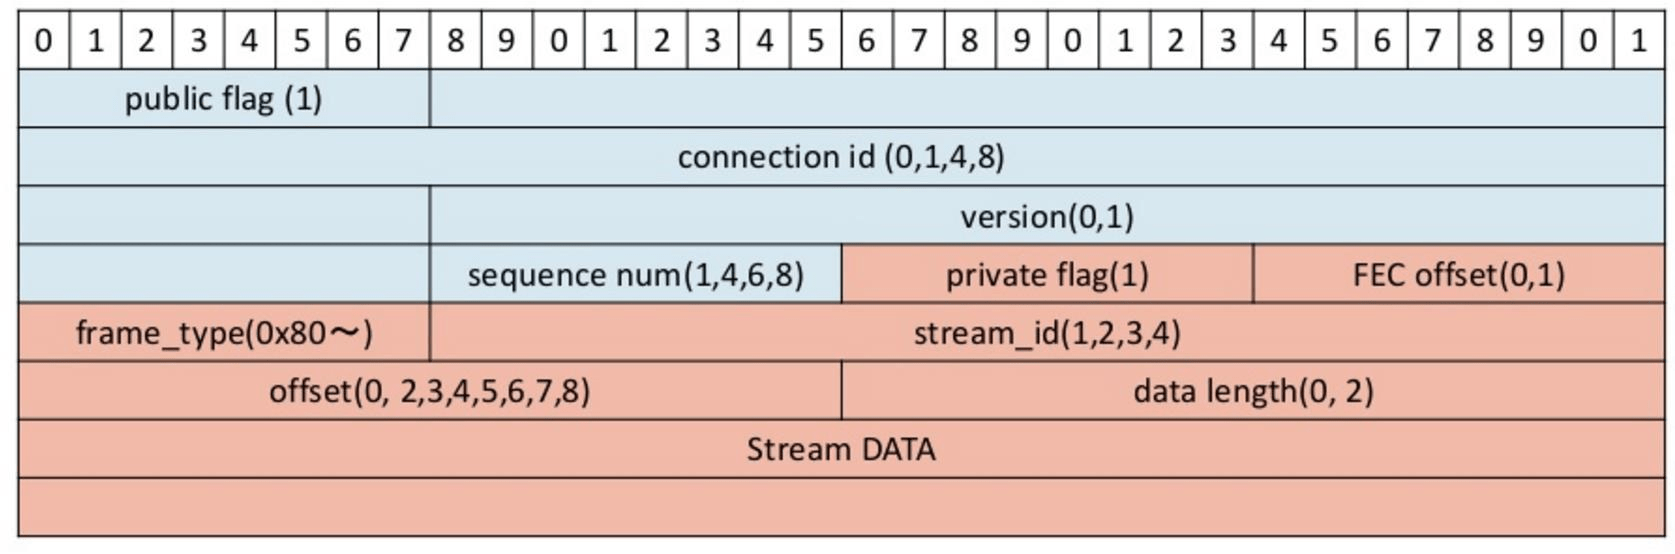
\includegraphics[width=1\linewidth]{quic_header.png}
    \caption{Hlavička QUIC. Spousta políček má proměnlivou velikost.}
\end{figure}

\begin{figure}[H]
    \centering
    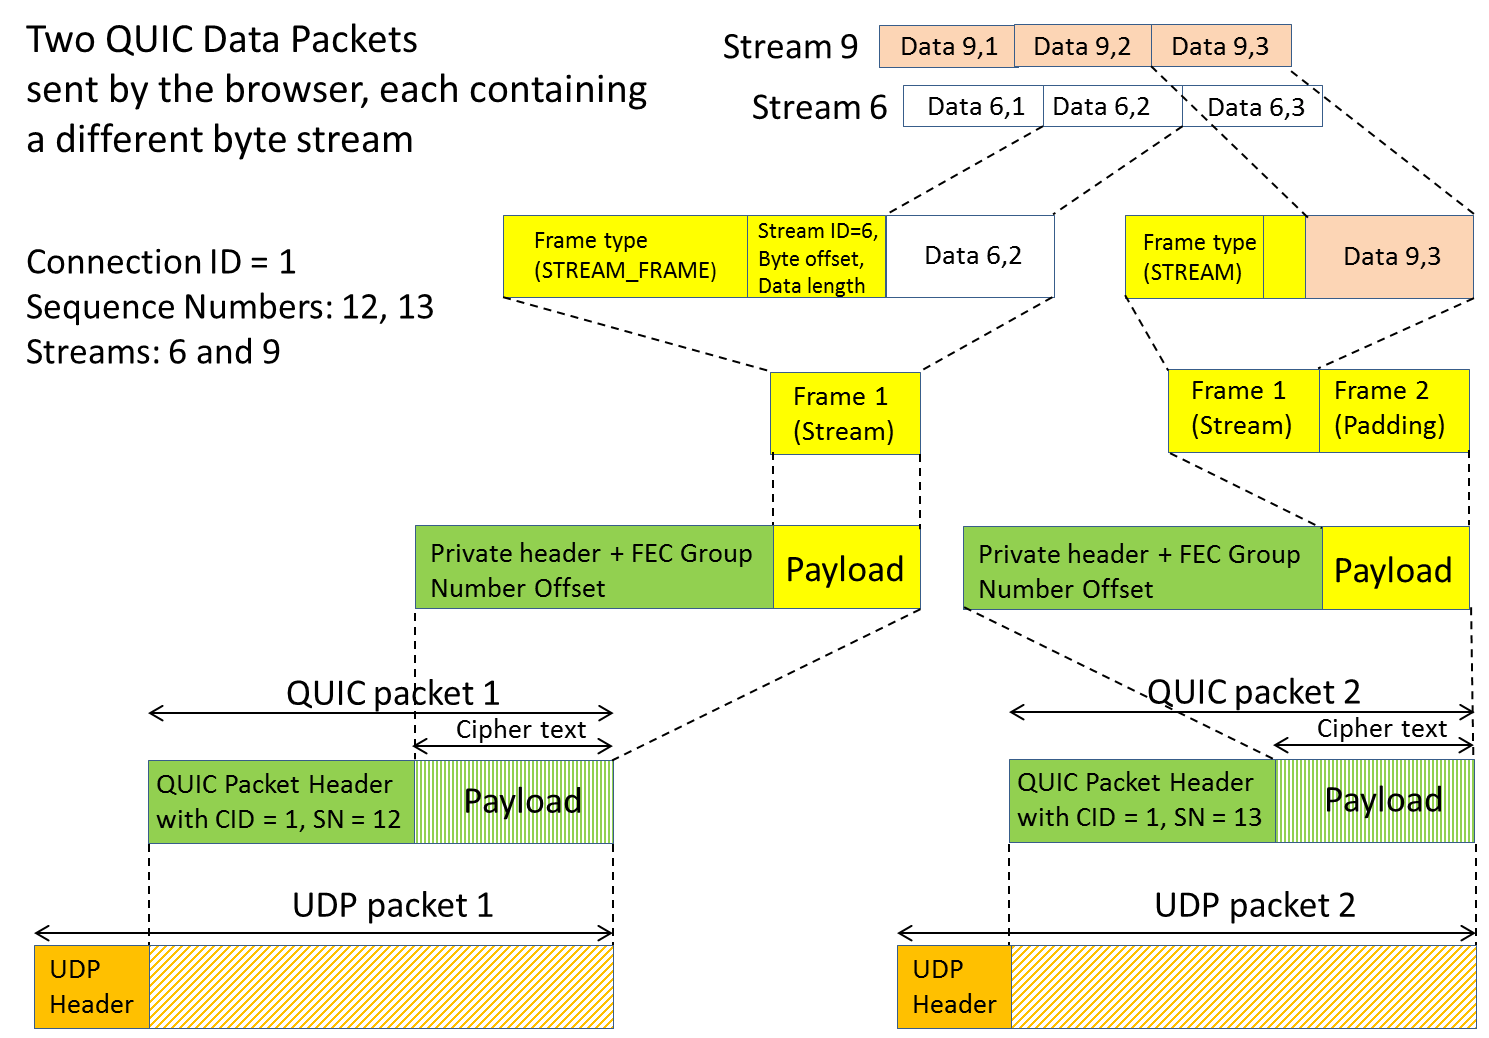
\includegraphics[width=1\linewidth]{quic_zprava.png}
    \caption{Složení QUIC zprávy.}
\end{figure}

% Rozlišuje mezi jednotlivými streamy jako SCTP
